\documentclass
[
a4paper,
german,
openright,                    % Kap.beginn immer rechts! (fkt. nur bei report, nicht bei article)
12pt                          % ersatzweise 12pt, wenn mehr Seiten entstehen sollen
]
{report}

%%%%%%%%%%%%%%%%%%%%%%%%%%%%%%%%%%%%%%%%%%%%%%%%%%%%%%%%%%%%%%%%%%%%%%%%%%%%%%%%%%%%%%%%%%%%%%%%%%%%%%%%%%%%
%Dokumenteneigenschaften

\newcommand{\Author}{Michael Pfn\"ur} 
\newcommand{\Title}{M\"oglichkeiten zur Einbindung von Single Board Computer  in ein bestehendes Fertigungsumfeld}
\newcommand{\Keywords}{KEYWORD 1, KEYWORD 2, KEYWORD 3, KEYWORD 4, KEYWORD 5}
\newcommand{\Advisor}{FH-Ass. Prof. Dipl. Phys. Judith Schwarzer}
\newcommand{\Birthdate}{22.02.1981}
\newcommand{\EnrolNum}{1310555048}
\newcommand{\VenueMonthYear}{Salzburg, Mai 2016}
\newcommand{\VenueDate}{Salzburg, am 15.05.2016}


%%%%%%%%%%%%%%%%%%%%%%%%%%%%%%%%%%%%%%%%%%%%%%%%%%%%%%%%%%%%%%%%%%%%%%%%%%%%%%%%%%%%%%%%%%%%%%%%%%%%%%%%%%%%
% Layout zusammengestellt von Richard Wanger im WS 2015/2016. Verschiedene Vorlagen wurden bei der Erstellung
% kombiniert und nach dem Masterleitfaden (Stand: Oktober 2015) adaptiert. Verwendung ohne Gewähr!

\usepackage{style}		%alle packages und Formatvorlagen befinden sich in dieser Datei


%%%%%%%%%%%%%%%%%%%%%%%%%%%%%%%%%%%%%%%%%%%%%%%%%%%%%%%%%%%%%%%%%%%%%%%%%%%%%%%%%%%%%%%%%%%%%%%%%%%%%%%%%%%%
% ORGANISATORISCHES

\begin{document}
\begin{titlepage}

\hspace{7cm}

\begin{center}
	{\Large\uppercase\expandafter{\bf Bachelorarbeit}}\\[0.5ex]
	\vspace{1cm}
	\Large{\bf\large \Title}\\
	\vspace{1.5cm}
	\normalsize durchgeführt am\\
	Studiengang Informationstechnik \& System--Management\\
	an der\\
	Fachhochschule Salzburg GmbH\\
\end{center}

\vspace{2cm}

\begin{center}
	\normalsize vorgelegt von
	\\
	{
		\Large{\bf\large \Author}\\
	}
	\vspace{2cm}
	
\includegraphics[width=7cm]{BilderAllgemein/Logo.jpg}\medskip
\end{center}
	
\vspace{2cm}

\begin{tabbing}
	\hspace*{3cm}\=\hspace*{4cm}\= \kill
	\> Studiengangsleiter: \> FH-Prof.~DI Dr. Gerhard Jöchtl \\*[0.2cm]
	\> Betreuer: \> \Advisor
\end{tabbing}

\vfill	

\begin{center}
\VenueMonthYear\\
\end{center}
\end{titlepage}
\chapter*{Eidesstattliche Erklärung}
\thispagestyle{plain}
\pagestyle{plain}

Hiermit versichere ich, Michael Pfnür, geboren am 22.Mai 1981, dass die vorliegende Bachelorarbeit von mir selbstständig verfasst wurde. Zur Erstellung wurden von mir keine anderen als die angegebenen Quellen und Hilfsmittel verwendet.
\vspace{3cm}

\VenueDate

\vspace{0.5cm}

\begin{tabular}{p{0.3\textwidth}p{0.32\textwidth}p{0.3\textwidth}}

\parbox[c]{1em}{
\includegraphics[width=5cm]{BilderAllgemein/Unterschrift.JPG}} &  &  \multicolumn{1}{c}{\EnrolNum} \\ \cline{1-1} \cline{3-3}

 \Author & & Matrikelnummer

\end{tabular}
\chapter*{Allgemeine Informationen}
\thispagestyle{plain}
\pagestyle{plain}

\begin{tabular}{p{0.3\textwidth}p{0.65\textwidth}}

Vor- und Zuname: & \Author \\*[0.2cm]
Institution: & Fachhochschule Salzburg GmbH \\*[0.2cm]
Studiengang: & Informationstechnik \& System-Management \\*[0.2cm]
Titel der Bachelorarbeit: & \Title \\*[0.2cm]
Schlagwörter: & \Keywords  \\*[0.2cm]
Betreuer an der FH: & \Advisor

\end{tabular}
\newpage

\section*{\Large\bfseries Kurzzusammenfassung}

Single Board Computer (SBC) sind Einplatinenrechner, bei denen die verschiedenen Hardware Komponenten auf einer Platine zusammengefasst sind.\\
Diese Arbeit beschäftigt sich mit dem Aufbau verschiedener Schaltungen zum Einsatz in einem bestehenden Fertigungsumfeld. Zunächst wird auf die unterschiedlichen Möglichkeiten zur Datenübertragung von SBCs und Sensoren eingegangen und einige verschiedenen Übertragungssysteme näher erörtert.\\
Im praktischen Teil der Arbeit werden drei Testszenarien für den Einsatze von SBCs beschrieben und auf die unterschiedlichen Möglichkeiten zur Datenspeicherung und Visualisierung eingegangen. Die Unterschiede, sowie die Vor- und Nachteile der einzelnen Varianten zur Datenspeicherung werden hier dargelegt.
\vspace{1cm}\\
\section*{\Large\bfseries Abstract}

Single Board Computers are computers where the different hardware is placed on one platin.\\
This paper concerned with the construction of several circuits in relation to an  application in existing production lines. First of all the capabilities of communication from SBCs and sensors  as well as different  telecommunication systems will be explained.\\
The practical part of this paper showes three test settings for the application of SBCs and discribes the various possibilities respectively to data storage and visualization. The variaties, advantages and disadvantages of the different versions will be presented.
\chapter*{Danksagung}
\thispagestyle{plain}
\pagestyle{plain}

Zunächst möchten ich mich an dieser Stelle bei all denjenigen bedanken, die mich während der Anfertigung dieser Bachelorarbeit unterstützt haben.\\

Ganz besonders danken möchten ich in erster Linie meiner Betreuerin, Frau FH-Ass.~Prof.~Dipl.~Phys.~Judith Schwarzer, für ihre ausgiebige Unterstützung. Durch stetiges Hinterfragen und konstruktive Kritik verhalf sie mir zu einer durchdachten Herangehensweise und Umsetzung. Dank ihrer Erfahrung konnte sie mich immer wieder bei meinen Recherchen und bei meinen Fragen unterstützen. Vielen Dank für Zeit und Mühen, die Sie in meine Arbeit investiert haben.\\

Auch möchten ich mich bei der Robert Bosch AG für die gegebene Möglichkeit dieses Projekt durchzuführen, sowie für das dazu benötigte Equipment, welches zur Verfügung gestellt wurde bedanken.\\ 


\newpage

%%%%%%%%%%%%%%%%%%%%%%%%%%%%%%%%%%%%%%%%%%%%%%%%%%%%%%%%%%%%%%%%%%%%%%%%%%%%%%%%%%%%%%%%%%%%%%%%%%%%%%%%%%%%
%VERZEICHNISSE

\tableofcontents
\protect \addcontentsline{toc}{chapter}{Inhaltsverzeichnis}

\renewcommand{\nomname}{Abkürzungsverzeichnis}
\chapter*{Abkürzungsverzeichnis}
\addcontentsline{toc}{chapter}{Abkürzungsverzeichnis} 
\pagestyle{plain}

\begin{acronym}[SQL]
 \acro{SPI}{Serial Peripheral Interface}
 \acro{SBC}{Single Board Computer}
 \acro{I$^2$C}{Inter-Integrated Circuit}
 \acro{I$^2$S}{Integrated Interchip Sound}
 \acro{CAN}{Controller Area Network}
 \acro{RPI}{Raspberry Pi}
 \acro{BLE}{Bluetooth Low Energy}
 \acro{CSI}{Camera Serial Interface}
 \acro{DSI}{Display Serial Interface}
 \acro{GPIO}{General Purpose Input\;/\;Output}
\end{acronym}

\listoffigures
\protect \addcontentsline{toc}{chapter}{Abbildungsverzeichnis}

\listoftables
\protect \addcontentsline{toc}{chapter}{Tabellenverzeichnis}

\lstlistoflistings
\protect \addcontentsline{toc}{chapter}{Listingverzeichnis}

%%%%%%%%%%%%%%%%%%%%%%%%%%%%%%%%%%%%%%%%%%%%%%%%%%%%%%%%%%%%%%%%%%%%%%%%%%%%%%%%%%%%%%%%%%%%%%%%%%%%%%%%%%%%
%INHALT
\chapter{Einleitung}

Ein häufig verwendetes Schlagwort heutzutage wenn über die industrielle Produktion gesprochen wird ist \textbf{Industrie 4.0}. Damit ist vornehmlich gemeint, dass viele Abläufe vollautomatisiert von statten gehen. Egal ob dies in der Produktion selbst, in der Logistik, bei der Materialbestellung oder auch beim Versand der Fall ist. Um diese Anforderungen zu bewerkstelligen werden immer neuere Technologien eingesetzt, in diesen Zusammenhang werden Produkte wie Kleinstrechner, sogenannte \textbf{\ac{SBC}} von immer größeren Interesse. Beispiele hierfür sind der \textbf{\glqq Raspberry Pi\grqq} oder auch der \textbf{\glqq Banana Pi\grqq}, um nur einmal zwei der bekanntesten zu nennen. Es gibt allerdings auch noch eine Vielzahl anderer Produkte von \acp{SBC} auf dem Markt.

Die Aufgabe dieser Arbeit bestand darin, die Möglichkeiten für einen Einsatz von solchen \acp{SBC} in einem bestehenden Produktionsumfeld zu erproben. Der Bereich für den Einsatz erstreckt sich von der Temperaturmessung in den einzelnen Maschinen einer Produktionslinie bis hin zur Temperaturmessung in Schaltschränke oder Serverräumen um etwaige zu hohe Temperaturen frühzeitig erkennen zu können und diesen entgegenzuwirken. Weiterhin sollten auch noch Möglichkeiten für den Einsatz von Feuchtigkeitssensoren oder Vibrationssensoren erarbeitet werden, um z.B. Aussagen über die Schwingungsbelastung von nahegelegenen vielbefahrenen Zugstrecken und deren eventuelle Auswirkung auf die Produktion tätigen zu können. Ein weiterer zu erarbeitender Punkt war unterschiedliche Möglichkeiten zu testen, um die von den Sensoren gelieferten Daten effektiv zu speichern und aufzubereiten.

Die Arbeit ist folgendermaßen gegliedert. In Kapitel zwei werden einige der sich auf dem Markt befindenden \acp{SBC} miteinander verglichen um deren Vor- und Nachteile darzulegen und die bestmögliche Variante für die gegebenen Anforderungen auswählen zu können. Weiterhin werden die in den folgenden Kapiteln verwendeten Fachbegriffe erklärt, um diese zu verstehen. Auch werden die im späteren Verlauf verwendeten Bussysteme zur Übertragung der Daten vom Sensor an den \acl{SBC} erläutert, sowie dessen Übertragungsprotokolle. Im dritten Kapitel dem praktischen Teil werden die verschiedenen Schaltungen von unterschiedlichen Sensoren, sowie den unterschiedlichen Möglichkeiten zur Speicherung und Visualisierung der Daten dargestellt. Dabei wird vor allem auf die Datenspeicherung mittels \textbf{mySQL} und mit dem \textbf{RRDTool} eingegangen. Im letzten, den vierten Kapitel werden die zuvor erlangten Ergebnisse noch einmal zusammengefasst und ein Ausblick auf die Verwendung von \acp{SBC} in den verschiedenen Einsatzbereichen für die Zukunft gegeben.
\chapter{Theoretischer Teil}
\label{chapter_TheoretischerTeil}
Dieses Kapitel befasst sich mit den theoretischen Grundlagen, die für den Einsatz von \acp{SBC} zur Datenerfassung mittels verschiedenen Sensoren nötig sind. In Abschnitt \ref{section_Begriffsdefiniton} werden die im weiteren Verlauf der Arbeit verwendeten Fachbegriffe erläutert, um die beschriebenen Zusammenhänge gut zu verstehen. Der Abschnitt \ref{section_Vergleich_SBC} behandelt die unterschiedlichen sich auf dem Markt befindenden \acp{SBC} mit ihren jeweiligen Vor- bzw. Nachteilen. Die verschiedenen Bussysteme wie z.B. der \ac{I$^2$C}  Bus werden in Abschnitt \ref{section_Bussysteme} erklärt und deren Funktionsweise erläutert. 


\section{Begriffsdefinition}
\label{section_Begriffsdefiniton}
Die in diesem Abschnitt beschriebenen Definitionen wurden, soweit nicht anders angegeben aus folgendem Dokument entnommen \citep{Bussysteme_in_der_Praxis}.

\subsection*{Single Board Computer}
Unter einem \textit{Single Board Computer} (\ac{SBC}) versteht man ein Computersystem, welches sich komplett auf einer einzigen Platine befindet. \acp{SBC} können fast die gleichen Aufgaben erledigen wie gewöhnliche Computer, allerdings sind die Einplatinen Rechner diesen in Hinblick auf die Hardwareausstattung doch um einiges unterlegen.

\subsection*{Bussysteme}
\textit{Bussysteme} sind Systeme, die verwendet werden zur seriellen Datenübertragung zwischen einen oder mehreren Komponenten. Beispiele hierfür sind der \ac{I$^2$C} Bus, der \ac{SPI} Bus oder auch der \ac{CAN} Bus. Eine genauere Beschreibung der einzelnen Bussysteme folgt in Abschnitt \ref{section_Bussysteme}.

\subsection*{Raspberry Pi}
Der \textit{\ac{RPI}} ist ein \ac{SBC}, der von der britischen \textit{Raspberry Pi Foundation} aus Komponenten von Android-Smartphones entwickelt wurde.

\subsection*{Raspbian}
\textit{Raspbian} ist ein Betriebssystem, welches auf der Linux Distribution Debian basiert und speziell auf den Raspberry Pi angepasst wurde.

\subsection*{RRDTool}
Das \textit{RRDTool} ist ein Programm, mit dem man Round-Robin Datenbanken erstellen kann. Diese Datenbanken eignen sich besonders gut für die Aufzeichnung von zeitlich fortlaufenden Datenreihen wie z.B. Temperaturmessungen oder Strommessungen. Die Datenbank liegt dabei in einem einzigen File auf dem Datenträger und hat ab dem Erstellen eine feste Größe, die sich auch bei vielen Messungen über einen längeren Zeitraum nicht vergrößert. 

\subsection*{General Purpose Input/Output}
Unter \textit{\ac{GPIO}} versteht man elektrische Kontakte, die zur Realisierung verschiedener Funktionen für elektronische Geräte verwendet werden. Eine genauere Erklärung erfolgt in Abschnitt \ref{subsection_GPIO} \citep{Raspberri_Pi_Handbuch}.
\subsection*{Python}
\textit{Python} ist eine Programmiersprache, die vor allem auf dem Raspberry Pi bevorzugt verwendet wird.
\subsection*{Bluetooth Low Energy}
\textit{\ac{BLE}} ist eine Funktechnologie, die es ermöglicht, dass sich Geräte in unmittelbarer Entfernung zueinander vernetzen lassen. Die Stromkosten bei \ac{BLE} sind um einiges geringe als bei herkömmlichen Bluetooth \citep{Bluetooth_Low_Energy}.
\subsection*{Windows 10 IoT}
\textit{Windows 10 IoT} ist eine \glqq abgespeckte\grqq Version von Windows 10, die auf Mobilen Geräten wie dem Raspberry Pi lauffähig ist. IoT steht dabei für \textit{Internet of Things} \citep{Raspberri_Pi_Handbuch}.
%Abschnitt Vergleich von SBCs 
\section{Vergleich von verschiedenen SBC}
\label{section_Vergleich_SBC}
In diesem Abschnitt werden einige der bekanntesten \acp{SBC}, die sich auf dem Markt befinden miteinander verglichen, um den bestmöglichen für die vorgegebenen Anforderungen auswählen zu können.
Wichtige Kriterien für die Auswahl sind, dass die Möglichkeit besteht verschiedene Betriebssysteme (Windows und Linux) mit dem jeweiligen Einplatinenrechner betreiben zu können, sowie die verbaute Hardware(Taktfrequenz des Chips, RAM-Speicher). Ein weiterer Punkt welcher von Bedeutung ist, ist die Unterstützung von verschiedenen Kommunikationsschnittstellen (\ac{I$^2$C}, \ac{SPI}, 1-Wire), um eine große Anzahl von Sensoren nutzen zu können. Eine Übersicht der einzelnen Komponenten der verschiedenen \acp{SBC} sind in den Tabellen \ref{Tabelle_Vergleich_SBC1} und \ref{Tabelle_Vergleich_SBC2} dargestellt.

%Tabelle 1
\begin{table}[H]
%\rowcolors{2}{black!10}{black!20}
\centering
\begin{tabular}{
llll
}
\toprule
\multicolumn{1}{p{3cm}}{\textit{\ac{SBC}}} & \multicolumn{1}{p{3.5cm}}{\textit{Operating System} } & \multicolumn{1}{p{1,5cm}}{\textit{RAM} }&\multicolumn{1}{p{3cm}}{ \centering\textit{CPU} }\\\midrule
Banana Pi & Linux, Android & 1 GB & ARM Cortex-A7, 1 GHz\\
&&&\\
Raspberry Pi2&Windows, Linux&1 GB&ARM Cortex-A7 900 MHz\\
&&&\\
Raspberry Pi3&Windows, Linux&1 GB&ARM Cortex-A53 1,2 GHz\\
&&&\\
BeagleBone Black & Linux & 512 MB & ARM Cortex-A8 1 GHz\\
&&&\\
HummingBoard i2eX & Linux, Android & 1 GB & ARM Cortex-A9 1 GHz\\
&&&\\
Intel Galileo Gen 2 & Windows, Linux & 256 MB & x86 Quark 400 MHz\\
&&&\\
Radxa Rock & Linux & 2 GB & ARM Cortex-A9 1,6 GHz\\
\bottomrule
\end{tabular}
\caption{Vergleich OS, RAM, CPU verschiedener SBCs}
\label{Tabelle_Vergleich_SBC1}
\end{table}

\begin{threeparttable}[H]
%\rowcolors{2}{black!10}{black!20}
\centering
\begin{tabular}{
llll
}
\toprule
\multicolumn{1}{p{3cm}}{\textit{\ac{SBC}}} & \multicolumn{1}{p{3.5cm}}{\textit{Communication} } & \multicolumn{1}{p{3cm}}{\textit{Networking} }&\multicolumn{1}{p{3cm}}{ \textit{GPIO} }\\\midrule
Banana Pi & I$^2$C, SPI & 1\;GigE & 80\\
&&&\\
Raspberry Pi2&I$^2$C, SPI&10/100\;Mbps&40\\
&&&\\
Raspberry Pi3&I$^2$C, SPI&10/100\;Mbps\tnote{1} &40\\
&&&\\
BeagleBone Black &I$^2$C, SPI&10/100\;Mbps&66\\
&&&\\
HummingBoard i2eX &I$^2$C, SPI&1\;GigE&8\\
&&&\\
Intel Galileo Gen 2 & I$^2$C, SPI&10/100\;Mbps&20\\
&&&\\
Radxa Rock & I$^2$C, SPI\tnote{2}&10/100\;Mbps&80\\
\bottomrule
\end{tabular}

\begin{tablenotes}\footnotesize
\item[1] mit WLAN on Board
\item[2] nur für Android
\end{tablenotes}

\caption{Vergleich Schnittstellen, Netzwerkverbindung, Anzahl GPIO Pins}
\label{Tabelle_Vergleich_SBC2}
\end{threeparttable}

Wie aus den Tabellen ersichtlich ist, unterstützen die meisten aktuellen \acp{SBC} das Betriebssystem Linux. Eine Anforderung für diese Projekt war allerdings, dass sowohl ein Linux System, wie auch ein Windows System auf dem Board lauffähig ist. Aus diesem Grund fiel die Wahl auf den \ac{RPI}\;3, da dieser beide Betriebssysteme unterstützt und auch bei den anderen betrachteten Aspekten wie \textit{RAM, CPU} etc. den meisten Boards ebenbürtig oder sogar überlegen ist. Ein weiterer wichtiger Entscheidungsgrund für den \ac{RPI}\;3 war, dass es für diesen eine sehr große Anzahl an unterstützten Sensoren gibt (Sensoren die mit einer elektrischen Spannung von 3,3\;$V$ - 5\;$V$) betrieben werden. Dies ermöglicht einen sehr weit gefächerten Einsatz des \ac{RPI}\;3 und ist für das vorgesehene Projekt von großer Bedeutung.

%%Kapitel Raspberry PI
\section{Raspberry Pi 3}
\label{section_Raspberry_Pi3}
Das folgende Kapitel beschreibt den Raspberry Pi 3 und befasst sich genauer mit den verbauten Komponenten, welche im weiteren Verlauf der Arbeit benötigt werden. 

\subsection{Allgemeine technische Daten}
\label{subsection_Allgemeine_technische_Daten}
Die im folgenden Information wurden, soweit nicht anders angegeben von der offiziellen Homepage der \textbf{Raspberry Pi Foundation} entnommen \citep{RaspberryPiHomePage}.\\
Der \ac{RPI} 3 ist ein Kreditkarten großer Einplatinenrechner, welcher aktuell an die \textit{sieben Million} Mal verkauft wurde \citep{RPI_Verkaufszahlen}. Dieser besitzt\dots
\begin{itemize}
\item einen 1.2\;GHz 64-bit quad-core ARMv8 CPU
\item 802.11n Wireless LAN
\item Bluetooth 4.1
\item \ac{BLE}
\item 4 USB Ports
\item 40 GPIO Pins
\item Full HDMI Port
\item Ethernet Port
\item \ac{CSI}
\item \ac{DSI}
\item Micro SD Karten Slot
\end{itemize}

Die aktuelle Version des Raspberry Pi, der \ac{RPI}\;3 ist in Abbildung \ref{Abb_Bild_RPI3} dargestellt.

\begin{figure}[!h] 
  \centering
     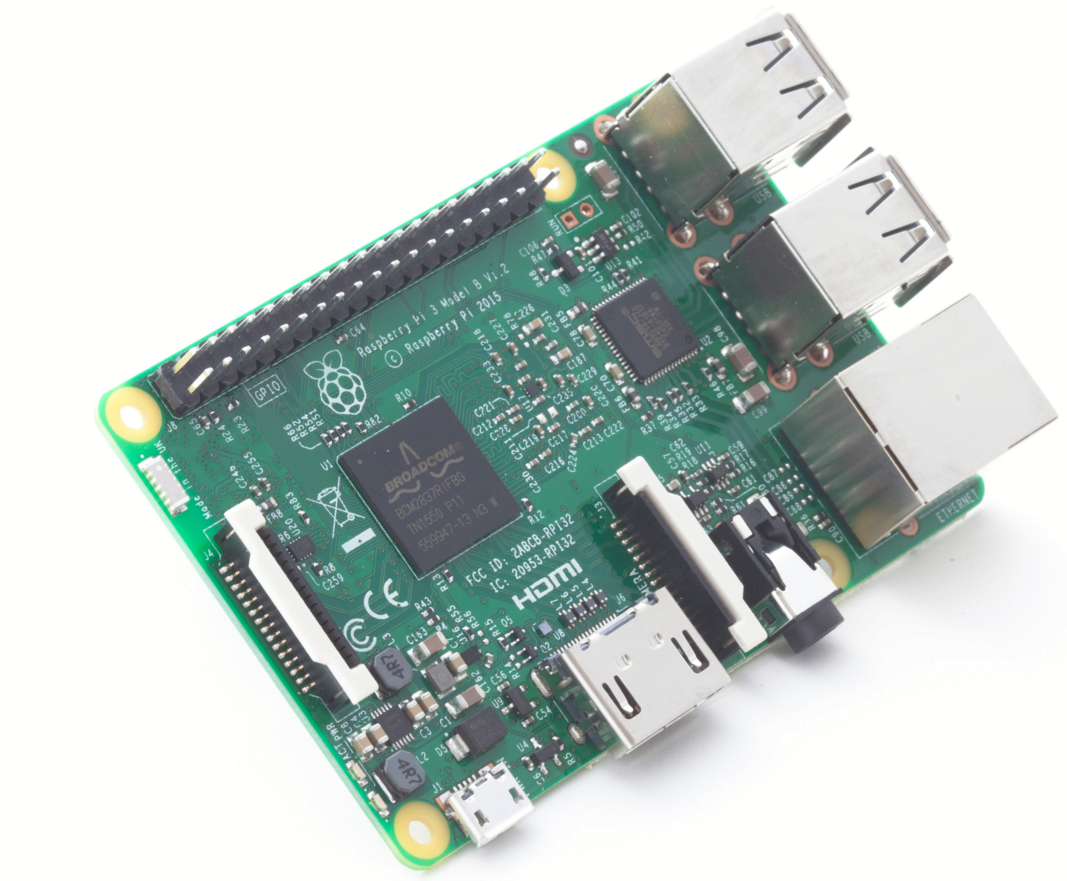
\includegraphics[scale=.4]{BilderAllgemein/RPI3.png}
  \caption{Raspberry Pi\;3 \citep{RPI_Bild}}
  \label{Abb_Bild_RPI3}
\end{figure}

Durch die im Gegensatz zu den Vorgänger Modellen leistungsstärkere CPU mit einem 64-Bit quad-core Prozessor, ist es beim RPI\;3 möglich das Windows Betriebssystem \textit{Windows 10 IoT} auf dem Gerät zu betreiben, wodurch sich eine Erweiterung der Einsatzmöglichkeiten (nicht mehr nur auf Linux Betriebssysteme beschränkt) ergibt. Auch wurde im Gegensatz zu den vorherigen Modellen beim aktuellen ein WLAN Modul (2,4\;GHz) gleich auf der Platine verbaut und muss nicht mehr extra durch ein externes USB-WLAN Modul realisiert werden. Der \ac{RPI}3 bietet weiterhin einen 10/100 MBit Ethernet Anschluss sowie einen \ac{CSI} und \ac{DSI} Anschluss zur direkten Anbindung einer Kamera oder Displays. Die verschiedenen GPIO-Pins werden in Kapitel \ref{subsection_GPIO} genauer beschrieben.

\subsection{GPIO-Kontakte}
\label{subsection_GPIO}
Wie bereits in Abschnitt \ref{subsection_Allgemeine_technische_Daten} angesprochen besitzt der \ac{RPI}\,3 40 GPIO-Kontakte, welche in einer Ecke der Platine zu 2\;x\;20 Kontakten angeordnet sind. Diese haben einen Rasterabstand von 2,54 mm zueinander und stellen die Grundlage für viele Projekte dar. Die ersten Modelle des \ac{RPI} besaßen dagegen nur 26 Pins die zur Verfügung standen. Die GPIO-Pins sind elektrische Kontakte, die zur Messung und Steuerung von elektronischen Geräten wie z.B. Sensoren, Analog Digital Wandlern, LEDs etc. verwendet werden.\\
Die Steckerleiste beinhaltet einige allgemein verwendbare Pins (\textit{=\;General Purpose Input\;/\;Output}), sowie zwei verschiedene Spannungsversorgungen (\textit{3,3\;V} und \textit{5\;V}) und Masse Anschlüsse (\textit{0\;V}). Weiterhin beinhaltet die Steckerleiste Kontakte für den \ac{I$^2$C}-, \ac{SPI}- und 1-Wire-Bus. Bei der Verwendung der GPIO-Kontakten für verschiedene Projekte, muss darauf geachtet werden, welche Bezeichnung verwendet wird. Diese ist in vielen Literaturen verschieden angegeben, da es drei verschiedene Möglichkeiten der Bezeichnung gibt. Die Benennung kann durch
\begin{itemize}
\item die physikalische Pin-Nummer, anhand seine Position auf dem Board (von oben gesehen, Pin 1 besitzt eine quadratische Lötstelle)
\item die BCM-Pin-Nummer, welche sich auf die Nummerierung der offiziellen Dokumentation des BCM2836-Chips bezieht
\item den Pin Namen, welcher von den \ac{RPI} Entwicklern vergeben wurde 
\end{itemize} 
vorgenommen werden \citep{Raspberri_Pi_Handbuch}.\\\\
In Abbildung ist die Pin Belegung des \ac{RPI} grafisch dargestellt.

%Grafik GPIO Pins
\begin{figure}[!h] 
  \centering
     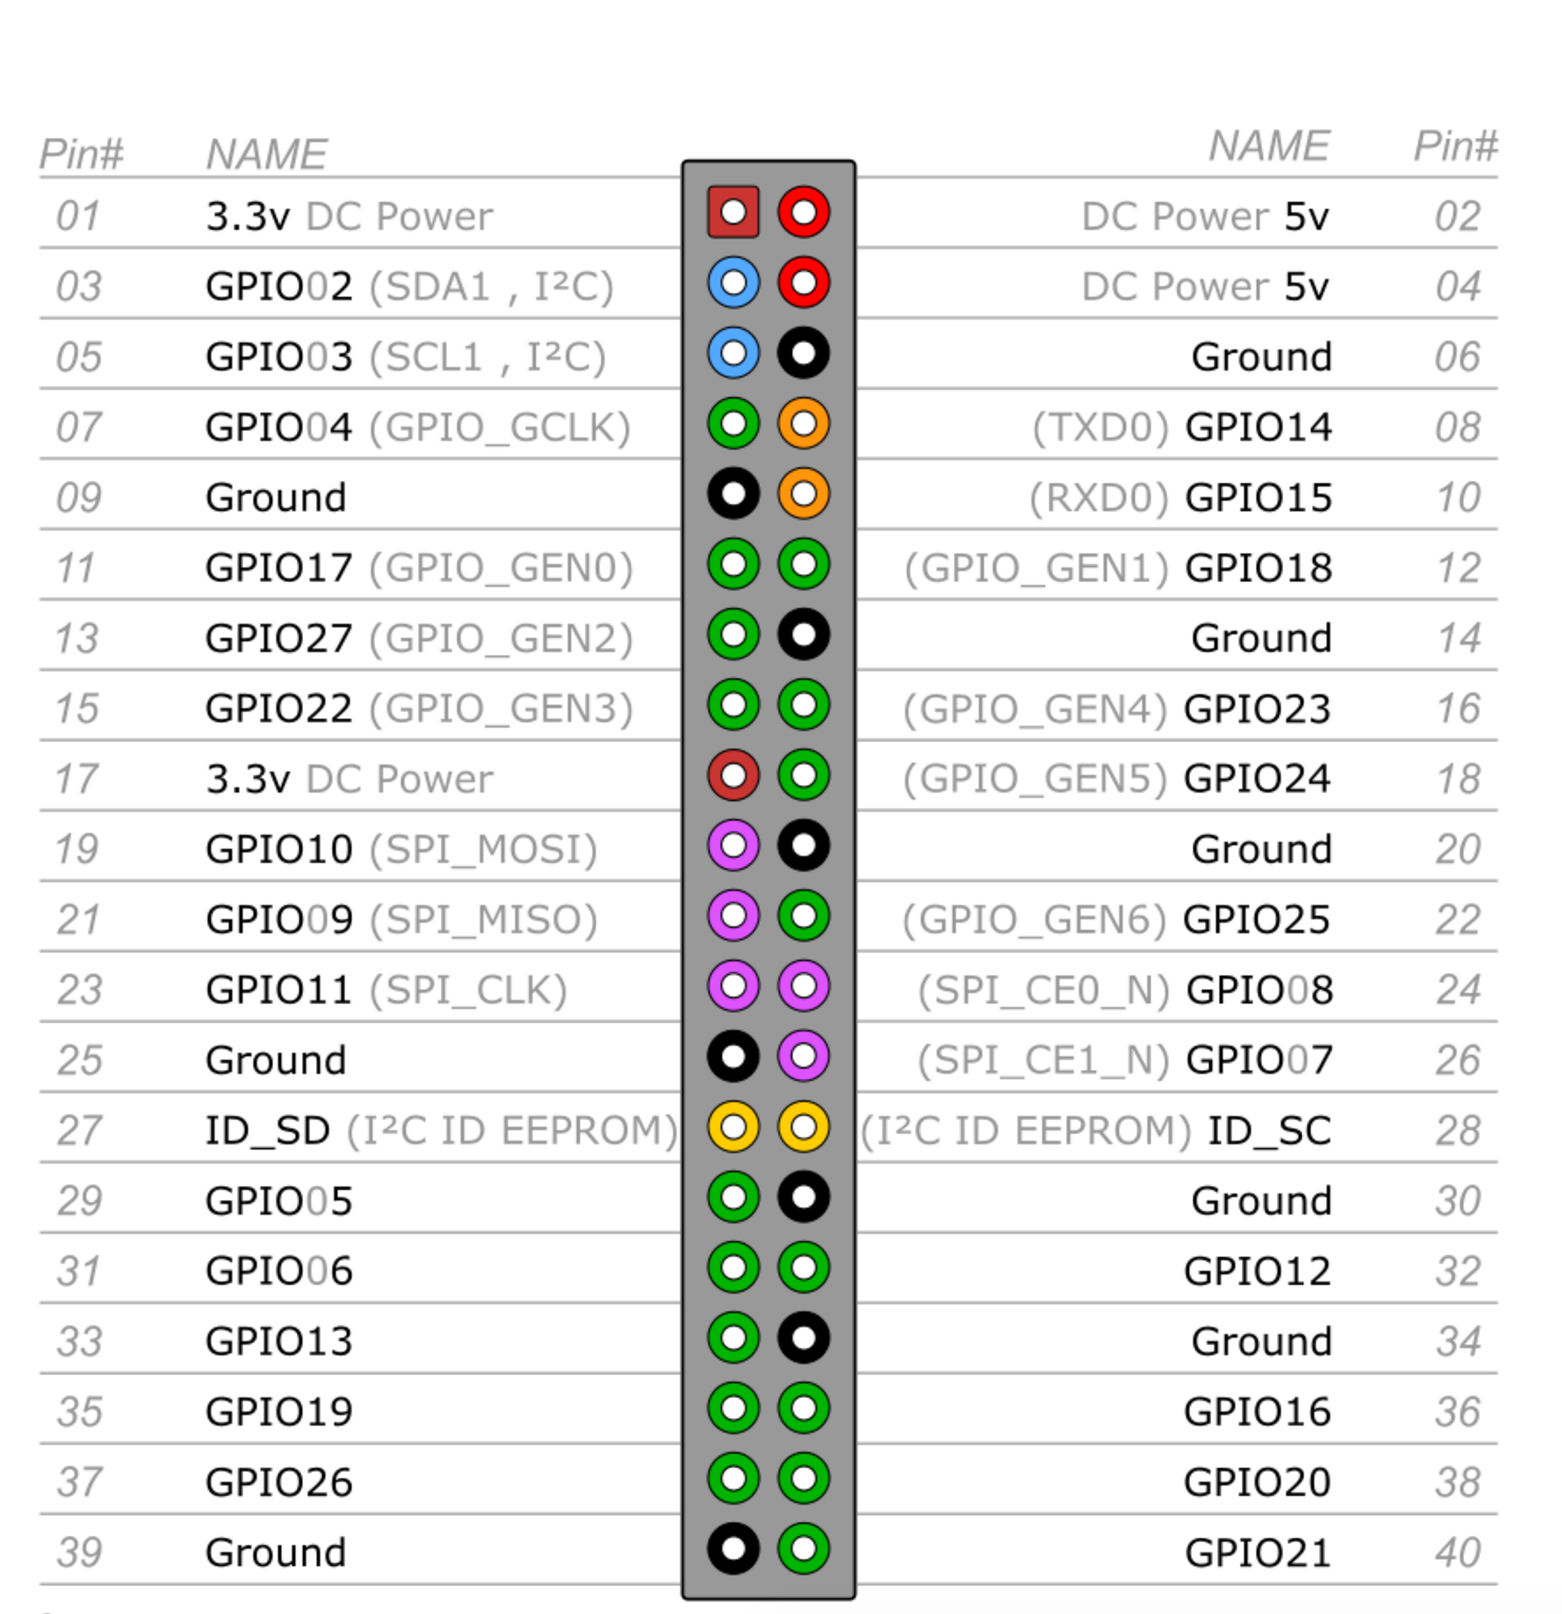
\includegraphics[scale=.35]{BilderAllgemein/GPIO.png}
  \caption{GPIO-Header \citep{GPIO_Header_Bild}}
  \label{Abb_Bild_GPIO}
\end{figure}

%% Section Bussysteme
\section{Bussysteme}
\label{section_Bussysteme}
Im folgenden Kapitel werden die am häufigsten verwendeten Bussysteme für die verschiedenen Sensoren erläutert. Zu diesen Bussystemen gehören der \textit{1-Wire}, \textit{\ac{I$^2$C}} und der \textit{\ac{SPI}} Bus. Auch wird auf die Funktion, sowie die Eigenheiten der Datenübertragung des jeweiligen Busses eingegangen.

\subsection{1-Wire}
\label{subsection_1Wire}
Der 1-Wire Bus ist ein serielles Bussystem von der Firma \textit{Dallas\footnote{2001 von Maxim Integrated übernommen}} , bei dem die Daten seriell (nacheinander) über eine Datenleitung übertragen werden.
\subsubsection{Allgemeine Informationen}
\label{subsection_Allgemeine_Informationen_1Wire}
 Für dieses Bussystem wird nur eine Datenleitung benötigt, die auch als Spannungsversorgung für den\;/\;die jeweiligen Sensoren benutzt wird. Physikalisch werden allerdings zwei Leitungen benötigt, da die Masse auch mitgeführt werden muss. Es gibt für diesen Bus eine große Anzahl an Sensoren wie z.B. Temperatursensoren, die sich durch einen sehr geringen Stromverbrauch auszeichnen. Dies kommt daher, da für die Datenübertragung und die Stromversorgung die gleiche Leitung genutzt wird, wird während der Kommunikation der Sensor aus einem internen Kondensator gespeist. Allerdings kann es notwendig sein, bei Sensoren wo die interne Spannungsversorgung nicht ausreichend ist  eine extra Spannungsversorgung für den jeweiligen Sensor mitzuführen. \\
Diese System ist ein \textit{One-Master-Multi-Slave} Bussystem, was bedeutet, dass es nur einen Master (z.B. \ac{RPI}) gibt aber mehrere Slaves (z.B. Sensoren). Die Aufgabe des Masters in diesem System ist es, die Kommunikation zu steuern. Die Anzahl der Sensoren kann bis zu 100 betragen, die parallel an den Master angeschlossen werden. Dies ist möglich, da jeder Sensor ein eindeutige 64 Bit lange ID besitzt. Diese gliedert sich in \citep{Bussysteme_in_der_Praxis}
\begin{itemize}
\item 8 Bit \textit{Family Code}
\item 48 Bit \textit{Seriennummer}
\item 8 Bit \textit{CRC-Prüfsumme}
\end{itemize}

\subsubsection{Übertragungsprotokoll}
\label{subsection_Protokoll_1Wire}
Der 1-Wire Bus wird dadurch, dass er keine Taktsignal benötigt als \textit{asynchroner} Bus bezeichnet. Dieser kommuniziert im \textit{Halbduplex} Verfahren, was bedeutet, dass immer nur ein Teilnehmer auf dem Bus senden oder empfangen kann (entweder Master oder ein Slave). Wenn keine Kommunikation stattfindet, wird die Datenleitung über einen Pullup-Widerstand auf \textit{high} gezogen und der in Abschnitt \ref{subsection_Allgemeine_Informationen_1Wire} erwähnte interne Kondensator geladen. In dem andern Fall wenn eine Übertragung stattfindet liegt die Datenleitung auf Masse und der Kondensator liefert in diesem Fall die Spannungsversorgung für den Sensor (abhängig vom Sensor siehe \ref{subsection_Allgemeine_Informationen_1Wire}). Da wie schon angesprochen keine Taktleitung vorhanden ist, muss für die Kommunikation ein bestimmter Ablauf eingehalten werden. Dafür gibt es zwei Übertragungsmöglichkeiten, den \textit{normalen Modus} wo ca. 16,3\;$kBit/s$ übertragen werden und den \textit{Overdrive Modus} mit bis zu 142\;$kBit/s$.\\
Die Zeitspanne für die Übertragung von 1 Bit beträgt immer 60\,$\mu s$. Diese Steuerung, egal in welche Richtung die Übertragung stattfindet werden durch den Master initiiert. Die Befehle die dazu notwendig sind, können aus der Tabelle \ref{Tabelle_Befehle_1Wire} entnommen werden \citep{Bussysteme_in_der_Praxis}.

%Tabelle 1
\begin{table}[H]
%\rowcolors{2}{black!10}{black!20}
\centering
\begin{tabular}{
llll
}
\toprule
\multicolumn{1}{p{2cm}}{\textit{Befehl} }&\multicolumn{1}{p{10cm}}{\centering\textit{Beschreibung} }\\\midrule
\textbf{Write 1} & Der Master zieht für $1-15\;\mu s$ auf Low. Der Rest des Slots bleibt \\
& ungenutzt.\\
&\\
\textbf{Write 0} & Der Master zieht den Bus für mindestens $60\;\mu s$ bis maximal\\
& $120\;\mu s$ auf Low.\\
&\\
\textbf{Read}& Der Master zieht für $1-15\;\mu s$ auf Low. Der Slave, der kommunizieren\\
& möchte, hält für eine 0 den Bus weiter auf Low. Will der Slave eine\\
& 1 senden, gibt er direkt den Bus wieder frei. Wie man leicht erkennt,\\
& ist der Status \textit{Write 1} oder Read für den Master gleich.\\
& Alleine der Status des Sensors bestimmt, ob ein Read oder Write 1 \\
& ausgeführt wird.\\
&\\
\textbf{Reset /} & Der Master zieht den Bus für min. $480\;\mu s$ auf Low. Wenn ein\\
\textbf{Presence} & Slave am Bus vorhanden ist, zieht er max. $60\;\mu s$ (also einen\\
& Slot) die Leitung auf Low. Somit weiß der Master, dass mindestens\\
& ein Slave angeschlossen ist.\\ 
\bottomrule
\end{tabular}
\caption{Befehle bei 1-Wire \citep[S. 35]{Bussysteme_in_der_Praxis}}
\label{Tabelle_Befehle_1Wire}
\end{table}

\subsection{I$^2$C-Bus}
\label{subsection_I2C}

\subsection{SPI-Bus}
\label{subsection_SPI}
\chapter{Praktischer Teil}
\label{chapter_Praktischer_Teil}
In diesem Kapitel werden die verschiedenen Sensorschaltungen und deren Konfiguration, die Problem
die sich bei der Realisierung ergaben, sowie die Ergebnisse und Auswertungen beschrieben. Außerdem werden die verschiedenen Möglichkeiten zur Datenspeicherung und Visualisierung dargestellt und erklärt. Am Anfang dieses Kapitels werden die zur Realisierung der verschiedenen Aufgaben benötigten Bauteile, kurz etwas näher erklärt und aufgelistet. In Abschnitt \ref{section_DS18S20} wird eine Schaltung mit einem einzigen 1-Wire Temperatursensor aufgebaut, bei der zweiten Schaltung in Abschnitt \ref{section_HTY221} kommt zu dem Sensor aus \ref{section_DS18S20} ein zweiter Temperatursensor und ein Sensor zur Temperaturmessung und Bestimmung der Luftfeuchtigkeit hinzu. Der letzte Abschnitt (\ref{section_BMA020}) befasst sich mit der Realisierung einer Vibrationsmessung mittels Beschleunigungssensors.

\section{Benötigte Materialien}
\label{section_Benötigte_Materialien}
Die in Tabelle aufgelisteten Materialien wurden für die in Kapitel \ref{chapter_Praktischer_Teil} beschriebenen Versuche verwendet. In den jeweiligen Abschnitten, werden die  einzelnen Sensoren mit deren wichtigsten Technischen Daten noch genauer erklärt. 

%Tabelle 1
\begin{table}[H]
%\rowcolors{2}{black!10}{black!20}
\centering
\begin{tabular}{
lc
}
\toprule
\multicolumn{1}{p{6cm}}{\textit{Bezeichnung}} & \multicolumn{1}{p{3.5cm}}{\centering\textit{Anzahl} } \\\midrule
Raspberry Pi\,3& 1 \\
&\\
Temperatursensor DS18S20 & 2 \\
&\\
Sensor HYT\,221 & 1\\
&\\
3-Achsen-Beschleunigungssensor & 1\\
&\\
Drahtbrücken & mehrere\\
&\\
elektrischer Widerstand 4.7\,$k\Omega$ & 1\\
&\\
Elektronik Steckbrett & 1\\
\bottomrule
\end{tabular}
\caption{benötigte Materialien}
\label{Tabelle_benötigte_Materialien}
\end{table}

%Abschnitt DS18S20
\section{Temperaturmessung mit Sensor DS18S20}
\label{section_DS18S20}
Abschnitt \ref{section_DS18S20} befasst sich mit dem Schaltungsaufbau zur Temperaturmessung mittels DS18S20. Weiterhin werden die verschiedenen Möglichkeiten zur Datenspeicherung (RRD Tool, mySQL), sowie eine Möglichkeit zur Visualisierung der Daten erläutert. 
 



\subsection{DS18S20}
\label{subsection_DS18S20}
Der DS18S20 (siehe Abbildung \ref{Abb_DS18S20}) ist ein digitaler 1-Wire Temperatursensor, der eine 9\,Bit Temperaturmessung ermöglicht. Dieser ist von der Firma \textit{Maxim Integrated} entwickelt worden.
Folgend werden die wichtigsten technischen Daten des DB18S20 aufgeführt.

%Abbildund Daten DS18S20
\begin{figure}[!h] 
  \centering
     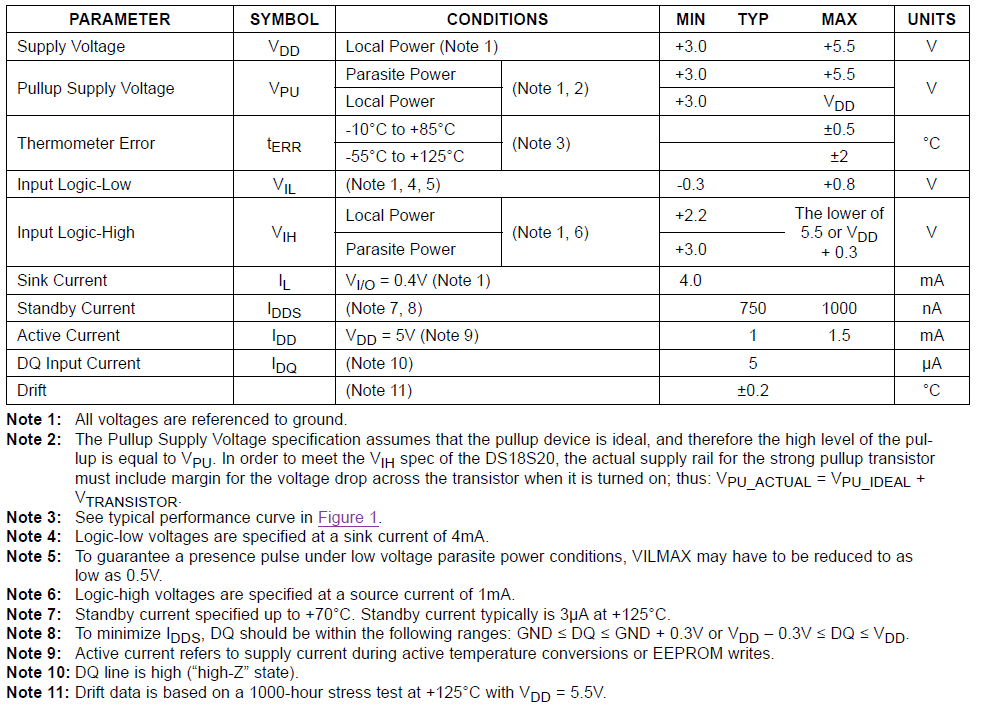
\includegraphics[scale=.6]{BilderAllgemein/Daten_DB18S20.png}
  \caption{elektische Daten DB18S20 \citep[S. 2]{Datenblatt_DB18S20}}
  \label{Abb_elektrische_Daten_DS18S20}
\end{figure}

%Abbildund  DS18S20
\begin{figure}[!h] 
  \centering
     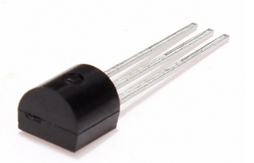
\includegraphics[scale=.4]{BilderAllgemein/DS18S20.png}
  \caption{DS18S20 \citep{Bild_DS18S20}}
  \label{Abb_DS18S20}
\end{figure}

\subsection{Schaltungsaufbau}
\label{subsection_Schaltungsaufbau_DS18S20}

Abbildung \ref{Abb_Schaltung_DS18S20} zeigt den schematischen Schaltungsaufbau mit dem Temperatursensor DS18S20. Anzumerken ist, dass die in der Schaltung in Abbildung \ref{Abb_Schaltung_DS18S20} dargestellten Bauteile optisch nicht immer den realen Bauteilen entsprechen (z.B. Aufdruck auf dem Sensor). Die Beschaltung der Bauteile wurde in der praktischen Erprobung ganz genau so durchgeführt. 

%Abbildund Schaltungsaufbau DS18S20
\begin{figure}[!h] 
  \centering
     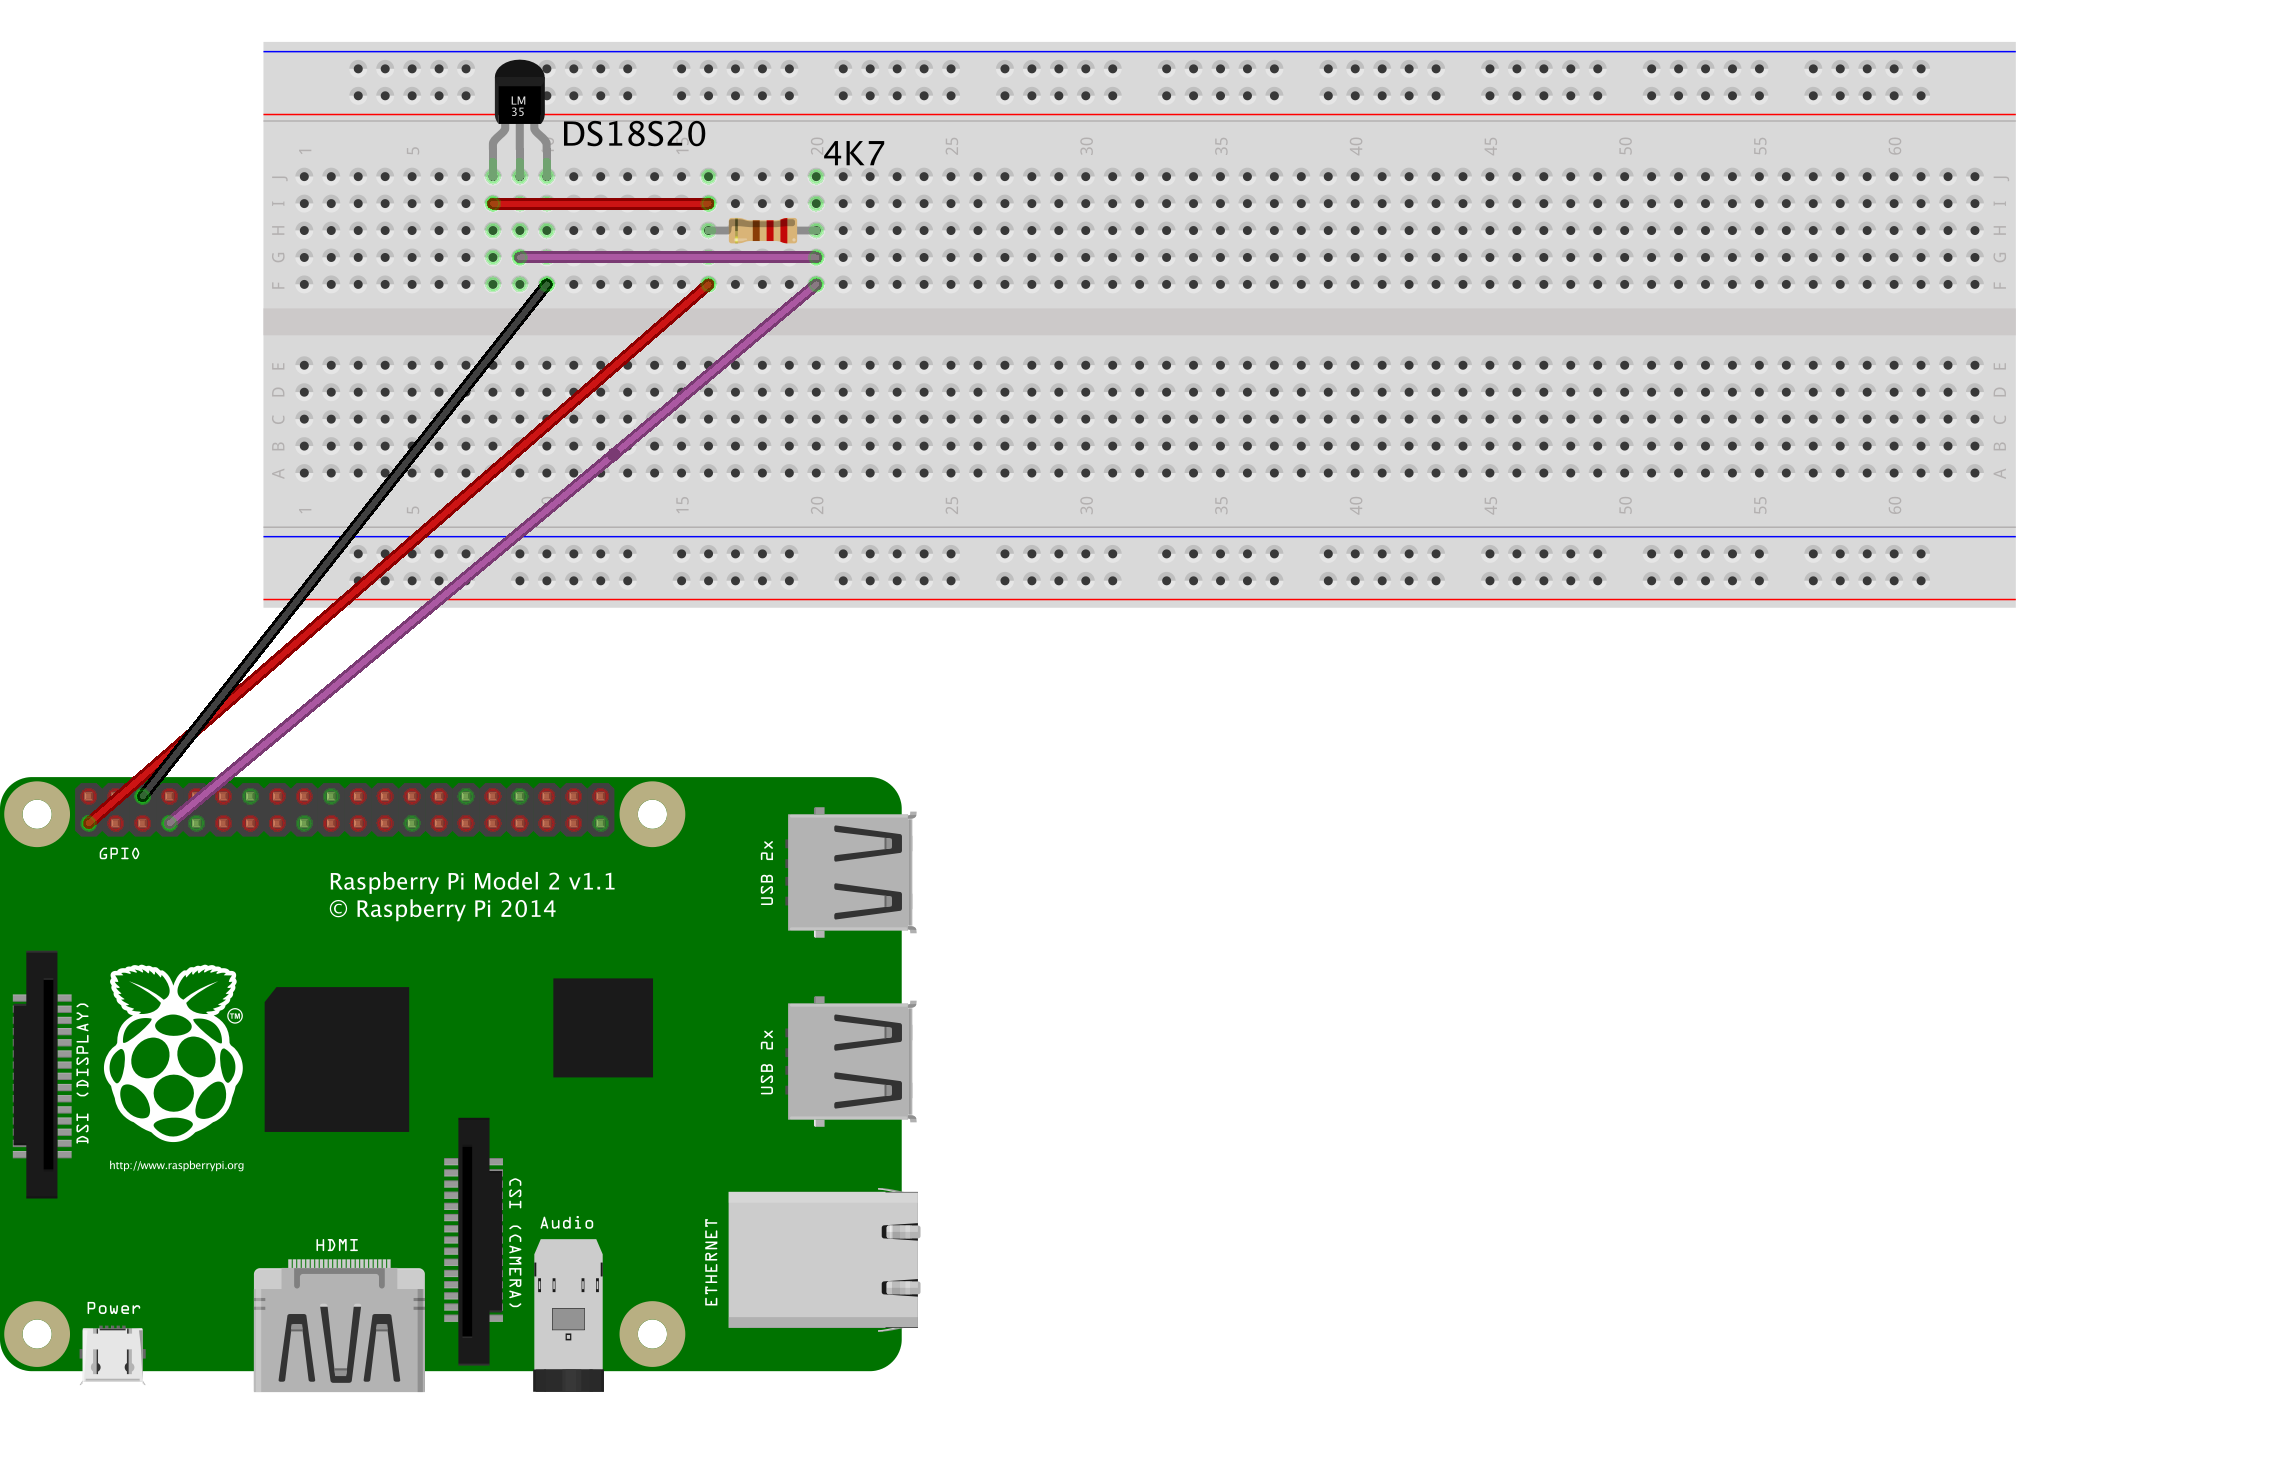
\includegraphics[scale=.8]{BilderAllgemein/Schaltung_DS18S20.png}
  \caption{Schaltungsaufbau DS18S20}
  \label{Abb_Schaltung_DS18S20}
\end{figure}

Die oben dargestellte Schaltung\footnote{gezeichnet mit Fritzing} zur Temperaturmessung wird folgendermaßen realisiert, der Pin $V_{DD}$ des Sensors ist mit Pin\,1 (3,3\,V) des \ac{RPI}\,3 verbunden (rote Verbindung). Die schwarze Verbindung stellt die GROUND Verbindung des Pin\,6 des \ac{RPI} mit dem GND Pin des Sensors dar. Weiterhin ist der er DQ Pin des Sensors (1-Wire Interface) mit dem Pin\,7 des \ac{RPI} verbunden (violette Verbindung) welcher für den 1-Wire Bus verwendet wird. Zu dem  $V_{DD}$ Pin  und dem DQ Pin ein Pullup Widerstand parallel geschalten.

\subsection{Auslesen des Sensors}
\label{subsection_Auslesen_DS18S20}
Um die vom Sensor erfassten Daten auf dem \ac{RPI}\,3 auszulesen, wird ein Python Script verwendet. Dieses wird im Anschluss an Hand kurzer Ausschnitte aus dem Quellcodes erklärt. Der komplette Quellcode ist im Anhand dieser Arbeit zu finden.\\

%Quellcode DS18S20
\lstset{escapeinside={\%*}{*},numbers=left,stepnumber=1}
\lstinputlisting[language=Python, firstline=16, lastline=32, caption=Auslesen der gemessenen Temperatur, label=list:Quellcode_DS18S20]{Listings/DS18S20/DS18S20.py}

Um die Temperatur des Sensors auslesen zu können wird als erstes das File wie in Zeile 2 des Codes ersichtlich ist geöffnet und dessen Inhalt in eine Variable gespeichert. Dieses File enthält die gesamten an den \ac{RPI}\,3 angeschlossenen IDs der 1-Wire Sensoren. Jeder angeschlossenen 1-Wire Sensor besitzt im Pfad \texttt{/sys/bus/w1/devices/} einen Ordner mit seiner ID. In diesem gibt es wiederum eine Datei mit der Bezeichnung \texttt{w1\_slave}, die die gemessenen Daten enthält. Um diese auszulesen, werden in unseren Python Script in den Zeilen $8-15$ verschiedene Schritte durchgeführt, auf die nicht näher eingegangen wird\footnote{kann in verschiedenen Python Tutorials nachgelesen werden}. Da die Temperatur in dieser Datei vom Sensor im Format von z.B. 17687 ($\approx$ 17,7 $^\circ$C) angegeben wird, muss dieser Wert noch durch 1000 dividiert werden um den genauen Temperaturwert zu erhalten(Zeile 15 im Quellcode). In Zeile 16 wird der Wert noch auf zwei Stellen nach dem Komma gerundet und ist in der Variable \texttt{temperature} gespeichert. Mit dem Wert dieser Variable kann nun weiter gearbeitet werden.

%Subsection Datenspeicherung
\subsection{Speicherung der Daten}
\label{subsectio_Datenspeicherung_DS18S20}
Wie schon in Abschnitt \ref{section_DS18S20} angesprochen, wird in dieser Arbeit auf zwei verschiedene Möglichkeiten der Datenspeicherung eingegangen. Zum Einen mit dem RRDtool und zum Andern mittels mySQL Datenbank. Die Möglichkeit der Datenspeicherung in einer mySQL Datenbank wird im Abschnitt \ref{section_HTY221} beschrieben. In diesem Abschnitt wird näher auf die Möglichkeiten mit dem RRDtool eingegangen.

\subsection*{RRDtool}
Unter dem RRDtool versteht man ein Programm, welches es ermöglicht, Messdaten für einen beim Erstellen festgelegten Zeitbereich zu speichern. RRD steht für \textit{Round-Robin-Database}, diese wird durch das Tool in einer Datei erzeugt, die von der Erstellung weg eine feste Größe besitzt. Dies ist ein großer Unterschied zu herkömmlichen mySQL Datenbanken, da bei diesen mit zunehmender Zeit und Datenmenge auch die Größe der Datenbank immer mit anwächst. Das Anwachsen der Größe der Datei wird bei der RRD Datenbank dadurch verhindert, dass sie wie ein Ringbuffer arbeitet. Dies bedeutet, dass wenn der Speicherplatz belegt ist, Werte zusammengefasst (z.B. durch Bildung eines Mittelwertes für einen Tag aus den einzelnen stündlichen Werten) und die ältesten überschrieben werden. Somit kann sichergestellt werden, dass die Größe der Datenbank schon beim Erstellen dieser festgelegt ist.\\
Wie eine solche Datenbank definiert und erstellt wird, wird im Quellcode beschrieben. Zum Erstellen der Datenbank wurde ein Shell-Script verwendet um nicht jedes Mal wenn die Datenbank neu erstellt wird alle Befehle einzeln eingeben zu müssen.

%Quellcode DS18S20
\lstset{escapeinside={\%*}{*},numbers=left,stepnumber=1}
\lstinputlisting[language=Python, firstline=1, lastline=9, caption=Erstellung RRD Datenbank , label=list:Quellcode_RRD_Datenbank]{Listings/DS18S20/RRD_DB_Erstellen.sh}
















\newpage
%Abschnitt HYT-221
\section{Temperatur- und Luftfeuchtigkeitsmessung mit HTY-221}
\label{section_HTY221}

\subsection{HYT-221}
\label{subsection_HYT221}
Der HYT-221 ist ein Sensor zur Messung der Temperatur und Luftfeuchtigkeit. Er wurde von der Schweizer Firma \ac{IST} für die Anwendung in den Bereichen Meteorologie, Industrielle Trocknungstechnik, Medizinische Geräte, Luftfahrt und Extremsport entwickelt. Der Sensor kommuniziert über eine \ac{I$^2$C} Schnittstelle und besitzt eine hohe Messgenauigkeit. In Tabelle \ref{Tabelle_Technische_Daten_HYT221}  werden die wichtigsten Daten des Sensors aufgelistet. Diese wurden dem Sensor zugehörigen Datenblatt entnommen \citep{Datenblatt_HYT221}.

%Tabelle Technische Daten HYT-221
\begin{table}[H]
%\rowcolors{2}{black!10}{black!20}
\centering
\begin{tabular}{
llll
}
\toprule
\multicolumn{2}{p{7cm}}{\centering\textbf{Feuchtemessung}} & \multicolumn{2}{p{7cm}}{\centering\textbf{Temperaturmessung} } \\
\multicolumn{1}{p{4cm}}{\textit{Bezeichnung}} & \multicolumn{1}{p{3cm}}{\centering\textit{Werte} }&\multicolumn{1}{p{4cm}}{\textit{Bezeichnung}} & \multicolumn{1}{p{3cm}}{\centering\textit{Werte} }\\\midrule
Messbereich & 0\dots 100\,\% rF & Messbereich  & -40\dots +125 $^\circ\text{C}$ \\
&&&\\
Genauigkeit & $\pm$ 1,8\,\% rF& Genauigkeit & $\pm$ 0,2 $^\circ\text{C}$\\
&&&\\
Auflösung & 0,02\,\% rF & Auflösung & 0.015 $^\circ\text{C}$\\
\bottomrule
\end{tabular}
\caption{Technische Daten HYT-221 \citep{Datenblatt_HYT221}}
\label{Tabelle_Technische_Daten_HYT221}
\end{table}

Für einen sicheren Betrieb des Sensors muss die angelegte Versorgungsspannung zwischen 2,7\dots 5,5\,$V$ liegen.

%Abbildund  HYT221
\begin{figure}[!h] 
  \centering
     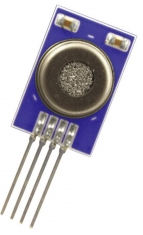
\includegraphics[scale=.8]{BilderAllgemein/HYT221.png}
  \caption{HYT-221 \citep{Bild_HYT221}}
  \label{Abb_HYT221}
\end{figure}




\section{Vibrationsmessung mit Sensor BMA020}
\label{section_BMA020}
\chapter{Zusammenfassung und Ausblick}
%\chapter{Beispiäle}

\thispagestyle{standard}
\pagestyle{standard}

\section{Text und Zitate}

In Moby-Dick geht es in erster Linie um die Jagd auf einen weißen Pottwal \footnote{nach: https://de.wikipedia.org/wiki/Moby-Dick}. Kurze Zitate (unter drei Zeilen) müssen mit Anführungszeichen gekennzeichnet werden. Außerdem müssen die Quelle sowie die Seite angegeben werden. Ein Beispiel für ein kurzes Zitat: \glqq Komisch. Manch einer von uns wünschte sich, er lebe auf einer Südseeinsel.\grqq \cite{MELVILLE:MOBYDICK1997} (Seite 100).

  \begin{quote}
"Das Buch hier Lieblingsbuch. Viele Blätter viele, schöne Bilder. Du kennen Worte?"\newline
"Ja"\newline
"Ich kennen Bilder. Das ein Wal. Du lesen Worte!"\newline
"Durch das Herz des Wals strömt mehr Flüssigkeit als durch das große Wasserleitungsrohr unter der London Bridge, jedoch strömt das Wasser nicht so stark, wie das Blut, das vom Herz des Wals pocht."\newline
"Du gut, ich danken dir."  \upshape \cite{MELVILLE:MOBYDICK1997} (Seite 500)
  \end{quote}

Ein sehr praktisches Package ist cleveref. Es automatisiert und erleichtert das setzen von Referenzen ungemein. Als Beispiel wird eine Referenz auf das FHS-Logo gesetzt siehe \cref{FIG_LOGO}.

Für das Verfassen von wissenschaftlichen Arbeiten können eine Vielzahl an Quellentypen herangezogen werden. Beispiele hierfür sind Leitfäden (Manuals) \citep{RFC2828} \citep{80211i} \citep{80211} \cite{X800} \citep{TR102377} \citep{EN301893} \citep{PUB197} \citep{PUB74}, Bücher \citep{Fis04a} \citep{Rei05a} \citep{Tan00a} \citep{Ste04a} \citep{GMS00a} \citep{HL98a}, Sammelbände \citep{EHL00a} \citep{Sch94a}, Journal-Artikel \citep{TM03a} \citep{CP03a}, Konferenz-Proceedings \citep{HCB00a} \citep{KBW04a} \citep{KSW04a} \citep{HK05a}, Internetmagazine \citep{Eke05a}, Webquellen \cite{nist} \cite{php} \cite{BDKMT93a} \cite{IDSSM} sowie Diplomarbeiten und Dissertationen \citep{Sch98} \cite{Hae94a}.

Als Beispiel für eine Abkürzung wird hier \ac{ADF} angeführt. Das Package schreibt automatisch das erste Vorkommen der Abkürzung aus. Die zweite Verwendung von \ac{ADF} wird also abgekürzt. Ist ein Ausschreiben einer Abkürzung gewünscht wird der acl-Befehl verwendet. Dies führt zu \acl{ADF}. Abkürzungen müssen in der Datei \glqq 05Abkuerzungsverzeichnis\grqq angegeben werden.

\section{Quelltext}

\texttt{printf("Hallo Welt")} für Ausschnitte von Sourcecode innerhalb von Text

\lstset{escapeinside={\%*}{*)},numbers=none}%oder numbers=left
\begin{lstlisting}[language=C,
caption=Beispiel-Listing,
label=LST_SAMPLE]
serverTCP = new TcpListener(IPAddress.Parse(serverIP), serverPort);
\end{lstlisting}

\lstset{escapeinside={\%*}{*)},numbers=left}
\lstinputlisting[language=Matlab, caption=Einfaches Matlabprogramm in einer Datei, label=list:hello.m]{Listings/hello.m}

\section{Bilder}

\begin{figure}[H]
\begin{center}
	
\includegraphics[scale=0.4]{BilderAllgemein/Logo.jpg}
\end{center}
	%\includegraphics[width=\textwidth]
	%\end{center}
	% Title
	\caption{Das FHS-Logo}
	% Unique name: identifier for referencing
	\label{FIG_LOGO}
\end{figure}

\section{Formeln}

Formeln sind für jeden Abschnitt rechtsbündig von dieser zu nummerieren, um einen späteren Bezug in der Arbeit zu gewährleisten. Formeln werden üblicherweise in "`Computer Modern Roman"' (\LaTeX{}-Standard) gesetzt. In diesem Template wird die Formel-Schrift bzw. das Package \texttt{eulervm} verwendet. Abgesetzte Formeln werden in \LaTeX{} durch die 
\emph{equation} Umgebung definiert. Formelausdrücke innerhalb von Textabschnitten erhält man durch \$Formel\$.

\subsection*{Beispiel}
%
Der \emph{Sinus cardinalis} oder sinc-Funktion ist eine mathematische Funktion $f$, welche in nicht-normierter Version als

\begin{equation}
	f(x) := \frac{\sin(x)}{x}
	\label{eq:bsp}
\end{equation}

definiert wird. In der digitalen Signalverarbeitung findet meistens nachfolgende normierte Version $\mathrm{si}(x)$ oder $\mathrm{sinc}(x)$ Anwendung \cite{x1}, \cite{x2}. Für eine Visualisierung dieser Funktionen siehe Abb.~\ref{FIG_LOGO}.

\begin{equation}
	f(x) := \frac{\sin(\pi x)}{\pi x}
	\label{EQ_SAMPLE}
\end{equation}

\section{Beispiel für Tabellen}
%
Es empfiehlt sich, für Tabellen die Standard-\LaTeX{}-Umgebung \emph{tabular} zu verwenden. Bei Bedarf können natürlich auch Erweiterungen (z.B.~\emph{tabularx} oder \emph{array}) zur Anwendung kommen. Eine mögliche Darstellung zeigt Tabelle \ref{Table_Sinc}.

\begin{table}[h!]%
	\begin{center}
		\begin{tabular}{|r|r|r|}
			\firsthline
			$x$&$\mathrm{sinc}(x)$&$\mathrm{sin}(x)$\\\hline\hline
			$-0.5$&0.6366&-0.4794\\\hline
			$0$&1.0000&0\\\hline
			$0.5$&0.6366&0.4794\\\hline
		\end{tabular}
		\caption{Zwei Werte der Sinc-Funktion}
		\label{Table_Sinc}
	\end{center}
\end{table}










%%%%%%%%%%%%%%%%%%%%%%%%%%%%%%%%%%%%%%%%%%%%%%%%%%%%%%%%%%%%%%%%%%%%%%%%%%%%%%%%%%%%%%%%%%%%%%%%%%%%%%%%%%%%
% LITERATURVERZEICHNIS

\interlinepenalty=10000 % Literatureinträge: Absätze zusammenhalten
\clearpage
\addcontentsline{toc}{chapter}{Literatur}
\singlespace
\bibliography{Michi}
\interlinepenalty=100

%%%%%%%%%%%%%%%%%%%%%%%%%%%%%%%%%%%%%%%%%%%%%%%%%%%%%%%%%%%%%%%%%%%%%%%%%%%%%%%%%%%%%%%%%%%%%%%%%%%%%%%%%%%%
% ANHÄNGE

\begin{appendix}
%\include{Anhang_Mathematik}                 % A
%\include{Anhang_FormatDerParameterdateien}  % B
%\chapter{Quellcode}
\section{Python Script DS18S20}
%Quellcode DS18S20
\lstset{escapeinside={\%*}{*)},numbers=left}
\lstinputlisting[language=Python, firstline=1, lastline=47, caption=Quellcode zum Auslesen des DS18S20]{Listings/DS18S20/DS18S20.py}
\newpage


\section{Erstellung Graphen DS18S20}
\label{Erstellung Graphen DS18S20}
%Quellcode DS18S20
\lstset{escapeinside={\%*}{*)},numbers=left}
\lstinputlisting[language=Python, firstline=1, lastline=47, caption=Quellcode Erstellung Temperaturgraphen DS18S20]{Listings/DS18S20/TemperaturGrafik.sh}
\newpage

\section{Python Script HYT-221 mit RRD}
\label{Python Script HYT-221 mit RDD}
\lstset{escapeinside={\%*}{*)},numbers=left}
\lstinputlisting[language=Python, firstline=1, lastline=128, caption=Quellcode zum Auslesen und Speichern der Daten von drei Sensoren mit RRDtool]{Listings/HYT221/Messung_RRD.py}
\newpage

\section{Python Script HYT-221 mit mySQL}
\label{Python Script HYT-221 mit mySQL}
\lstset{escapeinside={\%*}{*)},numbers=left}
\lstinputlisting[language=Python, firstline=1, lastline=126, caption=Quellcode zum Auslesen und Speichern der Daten von drei Sensoren mit mySQL DB]{Listings/HYT221/Messung.py}
\newpage

\section{Erstellung Graphen HYT-221}
\label{Erstellung Graphen HYT-221}
\lstset{escapeinside={\%*}{*)},numbers=left}
\lstinputlisting[language=Python, firstline=1, lastline=205, caption=Quellcode zum Erstellen der Graphen für die drei Sensoren]{Listings/HYT221/MessungGrafik.sh}
\newpage                 % C
%\include{Anhang_Datenblaetter}              % D
%\include{Anhang_Glossar}                    % E
\end{appendix}

\end{document}